%%%%%%%%%%%%%%%%%%%%%%%%%%%%%%%%%%%%%%%%%
% Short Sectioned Assignment LaTeX Template Version 1.0 (5/5/12)
% This template has been downloaded from: http://www.LaTeXTemplates.com
% Original author:  Frits Wenneker (http://www.howtotex.com)
% License: CC BY-NC-SA 3.0 (http://creativecommons.org/licenses/by-nc-sa/3.0/)
%%%%%%%%%%%%%%%%%%%%%%%%%%%%%%%%%%%%%%%%%

% \documentclass[paper=a4, fontsize=11pt]{scrartcl} % A4 paper and 11pt font size
\documentclass[11pt, a4paper]{book}
\usepackage[T1]{fontenc} % Use 8-bit encoding that has 256 glyphs
\usepackage[utf8]{inputenc}
\usepackage{fourier} % Use the Adobe Utopia font for the document - comment this line to return to the LaTeX default
\usepackage{listings} % para insertar código con formato similar al editor
\usepackage[spanish, es-tabla]{babel} % Selecciona el español para palabras introducidas automáticamente, p.ej. "septiembre" en la fecha y especifica que se use la palabra Tabla en vez de Cuadro
\usepackage{url} % ,href} %para incluir URLs e hipervínculos dentro del texto (aunque hay que instalar href)
\usepackage{graphics,graphicx, float} %para incluir imágenes y colocarlas
\usepackage[gen]{eurosym} %para incluir el símbolo del euro
\usepackage{cite} %para incluir citas del archivo <nombre>.bib
\usepackage{enumerate}
\usepackage{hyperref}
\usepackage{graphicx}
\usepackage{tabularx}
\usepackage{booktabs}

\usepackage[table,xcdraw]{xcolor}
\hypersetup{
	colorlinks=true,	% false: boxed links; true: colored links
	linkcolor=black,	% color of internal links
	urlcolor=cyan		% color of external links
}
\renewcommand{\familydefault}{\sfdefault}
\usepackage{fancyhdr} % Custom headers and footers
\pagestyle{fancyplain} % Makes all pages in the document conform to the custom headers and footers
\fancyhead[L]{} % Empty left header
\fancyhead[C]{} % Empty center header
\fancyhead[R]{Víctor Cabrita Gómez} % My name
\fancyfoot[L]{} % Empty left footer
\fancyfoot[C]{} % Empty center footer
\fancyfoot[R]{\thepage} % Page numbering for right footer
%\renewcommand{\headrulewidth}{0pt} % Remove header underlines
\renewcommand{\footrulewidth}{0pt} % Remove footer underlines
\setlength{\headheight}{13.6pt} % Customize the height of the header

\usepackage{titlesec, blindtext, color}
\definecolor{gray75}{gray}{0.75}
\newcommand{\hsp}{\hspace{20pt}}
\titleformat{\chapter}[hang]{\Huge\bfseries}{\thechapter\hsp\textcolor{gray75}{|}\hsp}{0pt}{\Huge\bfseries}
\setcounter{secnumdepth}{4}
\usepackage[Lenny]{fncychap}


\begin{document}

	% Plantilla portada UGR
	\begin{titlepage}
\newlength{\centeroffset}
\setlength{\centeroffset}{-0.5\oddsidemargin}
\addtolength{\centeroffset}{0.5\evensidemargin}
\thispagestyle{empty}

\noindent\hspace*{\centeroffset}\begin{minipage}{\textwidth}

\centering

\includegraphics[width=0.9\textwidth]{logos/logo_ugr.jpg}\\[1.4cm]

\textsc{ \Large TRABAJO FIN DE GRADO\\[0.2cm]}
\textsc{ GRADO EN INGENIERÍA INFORMÁTICA}\\[1cm]

{\Huge\bfseries Título \\}
\noindent\rule[-1ex]{\textwidth}{3pt}\\[3.5ex]
{\large\bfseries Subtítulo }
\end{minipage}

\vspace{2.5cm}
\noindent\hspace*{\centeroffset}
\begin{minipage}{\textwidth}
\centering

\textbf{Autor}\\ {Estudiante}\\[2.5ex]
\textbf{Director}\\ {Tutor(a)(es)}\\[2cm]

\includegraphics[width=0.3\textwidth]{logos/etsiit_logo.png}\\[0.1cm]
\textsc{Escuela Técnica Superior de Ingenierías Informática y de Telecomunicación}\\
\textsc{---}\\
Granada, Junio de 201x
\end{minipage}
\end{titlepage}


	% Plantilla prefacio UGR
	\thispagestyle{empty}

\begin{center}
{\large\bfseries Título \\ Subtítulo }\\
\end{center}
\begin{center}
Nombre Del Estudiante\\
\end{center}

%\vspace{0.7cm}

\vspace{0.5cm}
\noindent{\textbf{Palabras clave}: \textit{software libre}
\vspace{0.7cm}

\noindent{\textbf{Resumen}\\
	

\cleardoublepage

\begin{center}
	{\large\bfseries Same, but in English}\\
\end{center}
\begin{center}
	Student's name\\
\end{center}
\vspace{0.5cm}
\noindent{\textbf{Keywords}: \textit{open source}, \textit{floss}
\vspace{0.7cm}

\noindent{\textbf{Abstract}\\


\cleardoublepage

\thispagestyle{empty}

\noindent\rule[-1ex]{\textwidth}{2pt}\\[4.5ex]

D. \textbf{Tutora/e(s)}, Profesor(a) del ...

\vspace{0.5cm}

\textbf{Informo:}

\vspace{0.5cm}

Que el presente trabajo, titulado \textit{\textbf{Chief}},
ha sido realizado bajo mi supervisión por \textbf{Estudiante}, y autorizo la defensa de dicho trabajo ante el tribunal
que corresponda.

\vspace{0.5cm}

Y para que conste, expiden y firman el presente informe en Granada a Junio de 2018.

\vspace{1cm}

\textbf{El/la director(a)/es: }

\vspace{5cm}

\noindent \textbf{(nombre completo tutor/a/es)}

\chapter*{Agradecimientos}






	% Índice de contenidos
	\newpage
	\tableofcontents

	% Índice de imágenes y tablas
	\newpage
	\listoffigures

	% Si hay suficientes se incluirá dicho índice
	\listoftables 
	\newpage

	% Introducción 
	\chapter{Introducción}

Este proyecto es software libre, y está liberado con la licencia General Public License v3 \cite{gplv3}.

\section{Motivación}
Con la irrupción y popularidad de diferentes servicios de streaming como Netflix \cite{Netflix} o HBO \cite{HBO}, el catálogo de series que uno puede ver ya no se limita a las que echen por la televisión. Ante este vasto mar de opciones, surgen dos problemas:
\begin{enumerate}
    \item Con tantas opciones, no somos capaces de discernir las que nos podrían interesar, causando el efecto contrario, que nos pasemos horas buscando para al final no ver nada.
    \item Como seres sociales que somos, nos surge la imperiosa necesidad de saber qué series se han visto nuestros conocidos y conocer su opinión sobre las mismas, a la vez que contarles a ellos nuestra opinión sobre las que nos hemos visto.
\end{enumerate}

El primer problema es resuelto en cierta forma por webs que clasifican y/o puntúan las series del catálogo actual. El segundo, a día de hoy sigue sin ser resuelto y está más que demostrada su necesidad por los usuarios de Twitter \cite{Twitter}, en los innumerables hilos en los que exponen su opinión sobre las series que han visto a lo largo del año.
\begin{figure}[H]
	\centering	
	
\includegraphics[scale=0.25]{img/twitter-thread-1.png}
    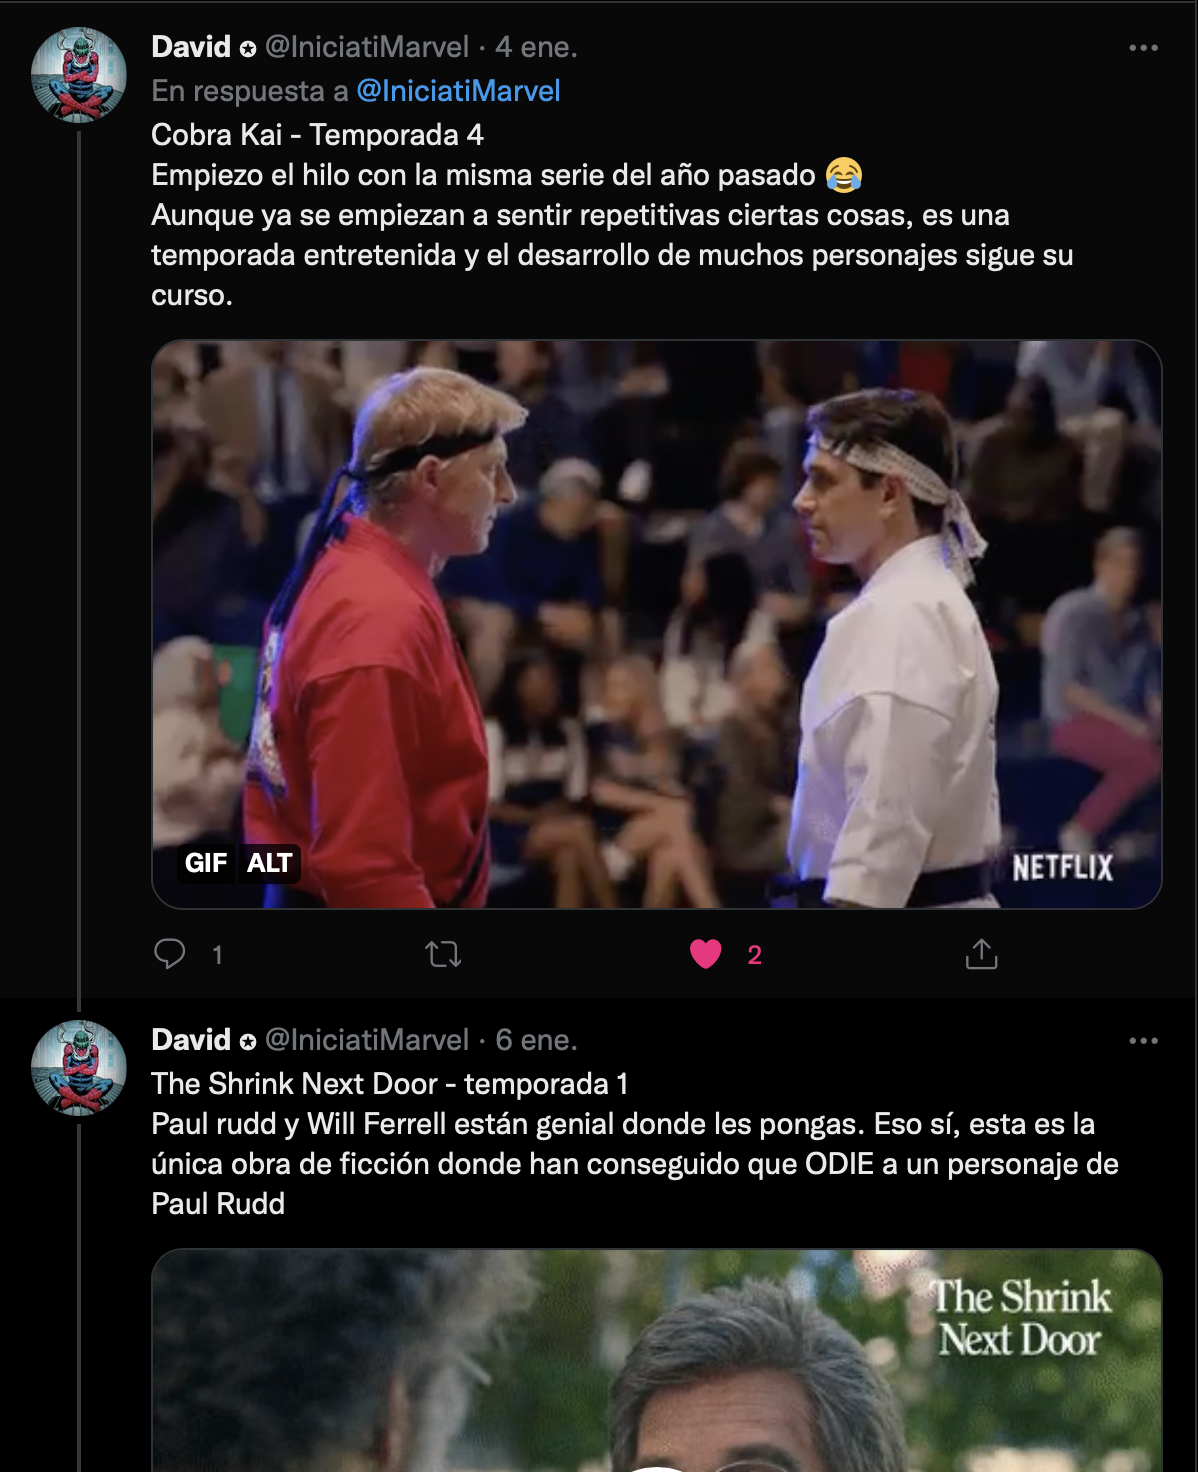
\includegraphics[scale=0.253]{img/twitter-thread-2.png}
	\caption{ @AcolyteJoel y @IniciatiMarvel, usuarios de Twitter, comentando su opinión sobre las series que han visto. }
    \label{fig:twitter_threads}
\end{figure}

\section{Objetivos}
El objetivo principal de este proyecto es crear una aplicación web en la que los usuarios puedan:
\begin{itemize}
    \item \textbf{Escribir} reseñas sobre las series que han visto.
    \item \textbf{Seguir} a otros usuarios para conocer su opinión sobre las series que éstos hayan visto.
    \item \textbf{Leer} reseñas de otros usuarios sobre las series que han visto.
\end{itemize}

Otro objetivo del proyecto, es desarrollar una versión móvil de la aplicación, para que los usuarios puedan hacer uso de la misma desde sus dispositivos móviles.

	% Descripción del problema y hasta donde se llega
	\chapter{Descripción del problema}



	% Estado del arte
	% 	1. Crítica al estado del arte
	% 	2. Propuesta
	\chapter{Estado del arte}

El software libre y sus licencias \cite{gplv3} ha permitido llevar a cabo una expansión del
aprendizaje de la informática sin precedentes.

	
	\chapter{Planificación}
Para empezar a desarrollar la solución al problema, primero hay que establecer la metodología de su desarrollo y
control de calidad.\\

\section{Metodología utilizada}
Para el desarrollo del proyecto, tenía claro que quería utilizar una metodología ágil\cite{agile}. Las metodologías
ágiles se basan en la aportación frecuente de código que tenga valor para el usuario. Esto permite una rápida
retroalimentación por parte de los usuarios y hace que el desarrollo sea muy flexible a posibles cambios en alguna
funcionalidad.\\

Las metodologías ágiles más utilizadas son Kanban y Scrum. Scrum se basa en ciclos cortos de trabajo en los que cada X
semanas, el cliente recibe un avance en el código de acuerdo a una previa planificación de los desarrolladores. Esta
metodología es perfecta para empresas, ya que facilita las reuniones con los clientes al fijar la duración de los
ciclos y les permite saber de antemano en qué están trabajando los desarrolladores en cada ciclo, sabiendo qué se van
a encontrar en la siguiente versión del proyecto y permitiéndoles influir en la planificación de los ciclos en base a
las funcionalidad más prioritarias para ellos. \\

Aunque la metodología SCRUM resulta muy útil cuando hay un cliente al que satisfacer con tiempos de entrega y para
planificar de acuerdo a unas prioridades las tareas a realizar por un equipo de trabajo. En este proyecto en el que no
hay un cliente, por lo que es flexible en cuanto a tiempos de entrega, y solo hay un desarrollador, no le estaría
sacando el máximo partido a la metodología SCRUM.\\

Por tanto, para el desarrollo del proyecto, se optado por seguir la metodología Kanban. Que permite un seguimiento
visual del proyecto en el que se puede ver en todo momento qué tareas se deben hacer, cuáles están en desarrollo y
cuáles se han terminado ya. Apoyándonos en una tabla Kanban los usuarios pueden ver en todo momento el estado del
proyecto y las nuevas funcionalidades en las que se está trabajando. \\
% TODO: Introducir tabla cuando avances con las HU

\subsection{Seguimiento del desarrollo}
Para la transparencia y visualización del proyecto a lo largo de sus diferentes fases, debemos de poder acceder a
estados anteriores en su desarrollo. Para ello, utilizaremos Git, un sistema de control de versiones, en el que
fácilmente podemos ver versiones anteriores del proyecto e incluso volver a ellas revirtiendo algunos cambios,
aumentando la adaptabilidad del proyecto a cambios en los requerimientos de los usuarios.\\

Para alojar el código y registrar las tareas a realizar se ha optado por GitHub, ya que con una cuenta de estudiante
nos da acceso a la creación de tableros Kanban, como el mostrado anteriormente, para la organización de las tareas y a
la integración continua, de la que hablaremos más adelante, a través de las GitHub Actions.

De esta forma, los \textit{stakeholders}, o personas interesadas en el desarrollo del proyecto, podrán ver en todo
momento en qué fase del desarrollo se encuentra el mismo, y en qué estado está cada una de sus funcionalidades.\\

\subsection{Milestones}
Las milestones son los productos mínimamente viables del proyecto. Están formadas por tareas más pequeñas que completan
el PMV.\\

Éstas tareas son:
\begin{itemize}
    \item \href{https://github.com/Torchu/flixbuff/labels/user%20story}{\textbf{Historias de Usuario}}. Requerimientos
    propuestos por los usuarios de la aplicación.
    \item \href{https://github.com/Torchu/flixbuff/labels/issue}{\textbf{Issues}}. Fallos o problemas en la aplicación
    que han de ser resueltos.
    \item \href{https://github.com/Torchu/flixbuff/labels/dev%20task}{\textbf{Tareas para el desarrollador}}. Pequeñas
    tareas que no representan una funcionalidad como tal.
\end{itemize}

Todas las tareas estarán asociadas a una issue diferente y tendrán una etiqueta acorde a su tipo.
\begin{figure}[H]
	\centering	
	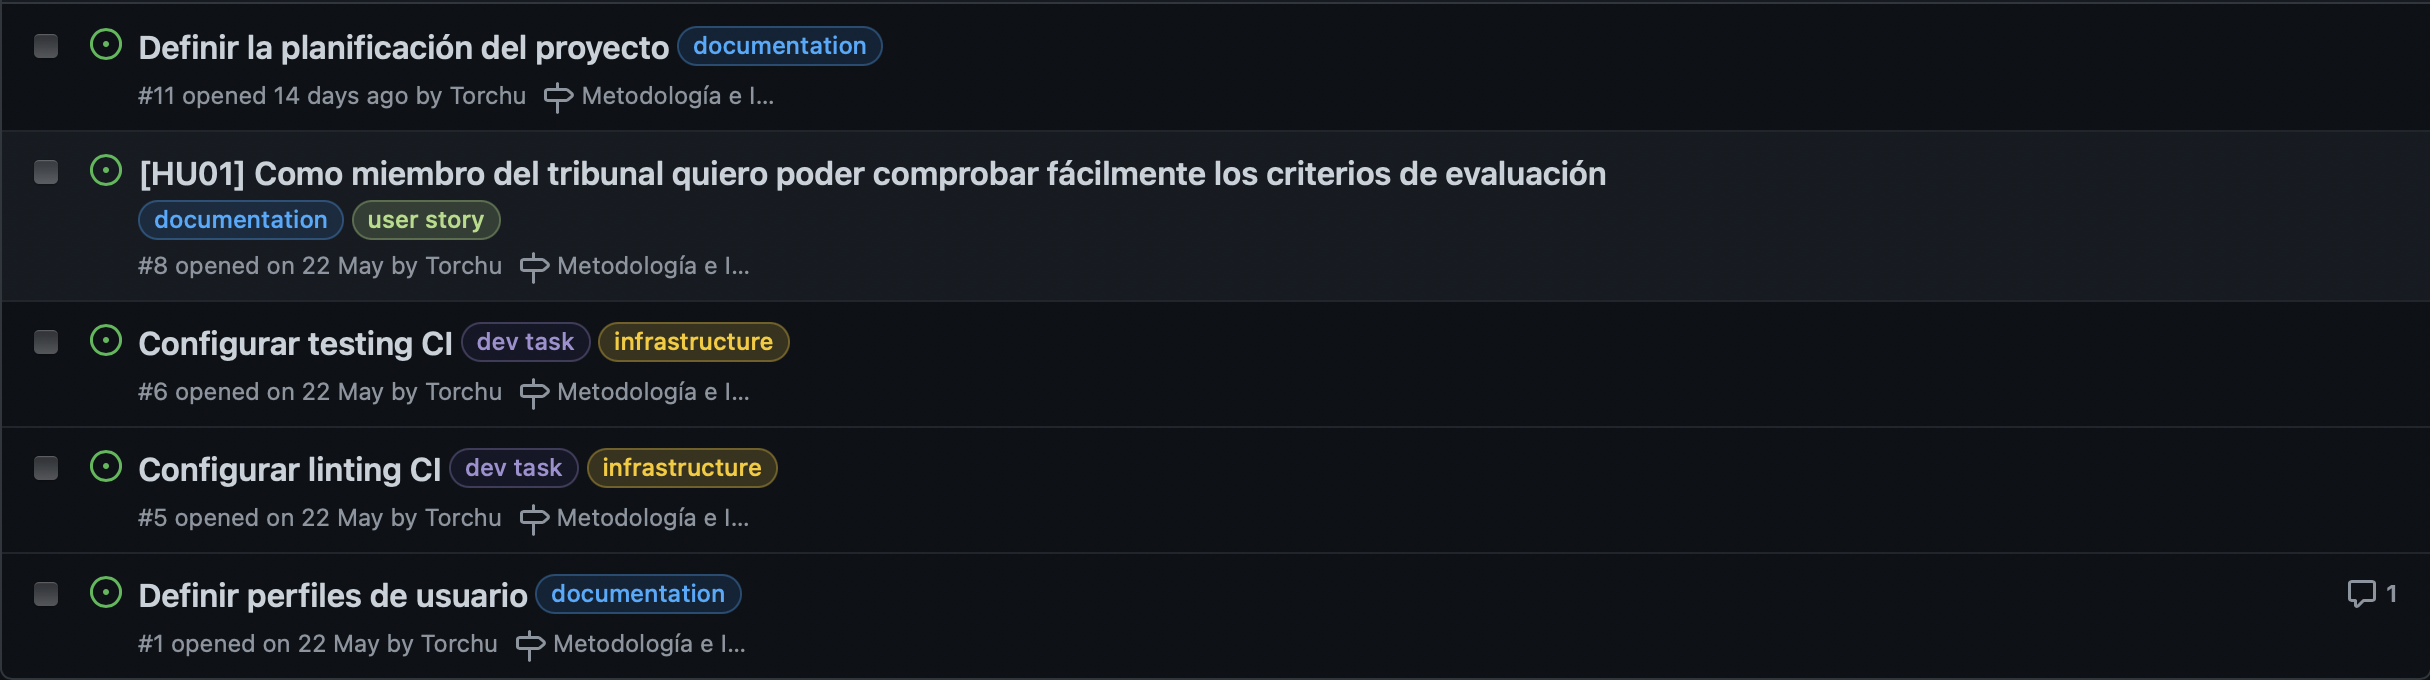
\includegraphics[scale=0.25]{img/issues.png}
	\caption{\href{https://github.com/Torchu/flixbuff/issues}{Issues} del proyecto}\label{fig:github_issues}
\end{figure}

Los milestones creados son visibles desde el repositorio de GitHub:
% TODO: Listarlos, poner links, etc.
% Son la infraestructura, el modelo de datos, el servicio de back y ambos front-end

\subsection{Historias de usuario}
Una historia de usuario es una funcionalidad que el usuario espera en la solución del problema. Es decir, un
requerimiento del usuario.\\

% TODO: Introducir imagen cuando avances con alguna HU

Como en este proyecto no tenemos unos usuarios que nos pidan los requisitos, se ha realizado un análisis de
\textit{Personas}\cite{personas}. Estas personas representan los perfiles de distintos usuarios de la aplicación y
serán ellos quienes protagonicen las historias de usuario. Ver \autoref{chap:personas}.\\

\section{Control de calidad}\label{sec:control_de_calidad}
Para asegurar la calidad del proyecto se ha seguido desde el comienzo del proyecto el desarrollo guiado por pruebas o
TDD\cite{TDD}.\\

Basándonos en esta metodología de desarrollo, trasladaremos los requisitos a una serie de pruebas dentro de nuestro
código, que se crearán antes del desarrollo de las funcionalidades. De esta forma, se convierten tanto en una
documentación fiable, que comprueba que el código desarrollado cumple los requisitos, como en una herramienta de
seguridad, que nos asegura que el código permanezca siempre correcto cada vez que se produzca algún cambio en el
mismo.\\
% TODO: Incluir imágenes de algún test

Además del desarrollo guiado por pruebas, se han configurado una serie de \textit{linters}. Unas herramientas que
comprueban que la sintáxis del código es correcta y cumplimenta la guía de estilo del lenguaje de programación en el
que está desarrollado, dando al desarrollador retroalimentación automática, reduciendo los costes de los posibles
cambios futuros, tal y como establece el dearrollo ágil.\\

Finalmente, se ha incluido un \textit{script} que comprueba la ortografía de toda la documentación del proyecto.\\

\subsection{Integración continua}

La integración continua es una metodología de trabajo que se basa en realizar integraciones frecuentes del código y
asegurarnos que superen los distintos controles de calidad.\\

Estos controles de calidad se comprueban mediante las \textit{pipelines}, o acciones que se ejecutan al subir código
al repositorio de GitHub. En nuestro caso incluiremos todo lo mencionado en el apartado
\hyperref{sec:control_de_calidad}{anterior}: pruebas de funcionalidad, \textit{linters} y revisión ortográfica.\\

Para este proyecto, se han configurado las \textit{pipelines} con la herramienta GitHub Actions. Se ha escogido esta
herramienta, ya que es propia de GitHub, la plataforma en la que se aloja el código del proyecto. Además, es muy fácil
de configurar. Simplemente incluyendo un fichero yaml en el directorio \textit{.github/workflows/} la propia plataforma
ya es capaz de reconocer y ejecutar las \textit{pipelines} que se han configurado.\\

% TODO: Incluir fotos aquí también cuando se hayan configurado el resto de GitHub Actions


	% Análisis del problema
	% 1. Análisis de requisitos
	% 2. Análisis de las soluciones
	% 3. Solucion propuesta
	% 4. Análisis de seguridad
	\chapter{Análisis del problema}
 


	% Desarrollo bajo sprints: 
	% 	1. Permitir registros y login de usuarios
	% 	2. Desarrollo del sistema de incidencias
	% 	3. Desarrollo del sistema de denuncias administrativas y accidentes
	% 	4. Desarrollo del sistema de croquis
	%   5. Instalación de la aplicación de manera automática
	\chapter{Implementación}

La implementación del software se ha dividido en hitos. Estos, han sido definidos en Github
y cada uno de ellos contiene un grupo de \textit{issues} que se corresponden con las distintas
mejoras que se han ido incorporando al software a lo largo de su desarrollo.\\



	% Presupuesto

	% Conclusiones
	\chapter{Conclusiones y trabajos futuros}



	% Trabajos futuros


	
	\newpage
	\bibliography{bibliografia}
	\bibliographystyle{plain}
	
\end{document}

